\chapter{Anhang}
\label{Anhang}

\section{Druckparameter}

\begin{table}[h]
    \centering
    \caption{Parametertabelle Prusa MK3S+\newline verwendet für Druck der Würfel und liegenden Zugproben}
      \begin{tabular}{llr}
      \toprule
      \textbf{Parameter} & \textbf{Wert} & \multicolumn{1}{l}{\textbf{Beschreibung}} \\
      \midrule
      Schichthöhe [mm] & \multicolumn{1}{r}{0,1} &  \\
      Drucktemperatur [°C] & \multicolumn{1}{r}{130} &  \\
      Druckgeschwindigkeit [mm/s] & \multicolumn{1}{r}{50} & \multicolumn{1}{p{12.555em}}{Liefert optisch gute Ergebnisse} \\
      Heizbetttemperatur [°C] & \multicolumn{1}{r}{40} &  \\
      Rückzugslänge [mm] & \multicolumn{1}{r}{0,6} & \multicolumn{1}{p{12.555em}}{Standardwert Cura} \\
      Materialflussrate [\%] & \multicolumn{1}{r}{100} &  \\
      Druckoberfläche & Flachkreppband & \multicolumn{1}{p{12.555em}}{Gute Ablöseeigenschaften mit Spachtel} \\
      Prozentsatz Aussenhaut überlappen [\%/mm] & 10/0,04 &  \\
      \bottomrule
      \end{tabular}%
    \label{Würfelparameter}%
  \end{table}


\section{Messwerte}

\begin{table}[h]
    \centering
    \caption{Abmaße, Volumen, Gewicht und Dichte der Würfel als Grünteil}
      \begin{tabular}{crrrrrrr}
      \toprule
      \textbf{Nr.} & \multicolumn{1}{l}{\textbf{h [mm]}} & \multicolumn{1}{l}{\textbf{l1 [mm]}} & \multicolumn{1}{l}{\textbf{l2[mm]}} & \multicolumn{1}{l}{\textbf{V [mm3]}} & \multicolumn{1}{l}{\textbf{V [cm3]}} & \multicolumn{1}{l}{\textbf{m [g]}} & \multicolumn{1}{l}{\textbf{Dichte [g/cm3]}} \\
      \multicolumn{1}{r}{1} & 10,03 & 10,13 & 10,2  & 1036,36 & 1,0364 & 4,775 & 4,607 \\
      \multicolumn{1}{r}{1} & 10,01 & 10,12 & 10,2  & 1033,27 & 1,0333 & 4,765 & 4,612 \\
      \multicolumn{1}{r}{1} & 10,02 & 10,15 & 10,17 & 1034,32 & 1,0343 & 4,76  & 4,602 \\
      \multicolumn{1}{r}{1} & 10,04 & 10,14 & 10,19 & 1037,40 & 1,0374 & 4,761 & 4,589 \\
      \multicolumn{1}{r}{1} & 10,03 & 10,15 & 10,19 & 1037,39 & 1,0374 & 4,76  & 4,588 \\
      \multicolumn{1}{r}{1} & 10,05 & 10,15 & 10,14 & 1034,36 & 1,0344 & 4,768 & 4,610 \\
      \multicolumn{1}{r}{1} & 10,06 & 10,13 & 10,19 & 1038,44 & 1,0384 & 4,751 & 4,575 \\
      \multicolumn{1}{r}{1} & 10,03 & 10,16 & 10,16 & 1035,35 & 1,0354 & 4,763 & 4,600 \\
      \multicolumn{1}{r}{1} & 10,02 & 10,17 & 10,16 & 1035,34 & 1,0353 & 4,762 & 4,599 \\
      \textbf{\textbf{$\varnothing$}} & \textbf{10,03} & \textbf{10,14} & \textbf{10,18} & \textbf{1035,80} & \textbf{1,0358} & \textbf{4,7628} & \textbf{4,5982} \\
      \midrule
      \multicolumn{1}{r}{2} & 9,94  & 10,22 & 10,2  & 1036,19 & 1,0362 & 4,724 & 4,559 \\
      \multicolumn{1}{r}{2} & 10,01 & 10,2  & 10,22 & 1043,48 & 1,0435 & 4,731 & 4,534 \\
      \multicolumn{1}{r}{2} & 9,97  & 10,18 & 10,22 & 1037,27 & 1,0373 & 4,754 & 4,583 \\
      \multicolumn{1}{r}{2} & 9,93  & 10,16 & 10,18 & 1027,05 & 1,0270 & 4,741 & 4,616 \\
      \multicolumn{1}{r}{2} & 9,97  & 10,21 & 10,22 & 1040,33 & 1,0403 & 4,751 & 4,567 \\
      \multicolumn{1}{r}{2} & 9,95  & 10,21 & 10,22 & 1038,24 & 1,0382 & 4,737 & 4,563 \\
      \multicolumn{1}{r}{2} & 9,95  & 10,15 & 10,23 & 1033,15 & 1,0332 & 4,741 & 4,589 \\
      \multicolumn{1}{r}{2} & 9,94  & 10,21 & 10,17 & 1032,13 & 1,0321 & 4,738 & 4,591 \\
      \textbf{\textbf{$\varnothing$}} & \textbf{9,96} & \textbf{10,19} & \textbf{10,21} & \textbf{1035,98} & \textbf{1,0360} & \textbf{4,7396} & \textbf{4,5751} \\
      \bottomrule
      \end{tabular}%
    \label{Grünteilmaße}%
  \end{table}%
  \FloatBarrier
  \begin{table}[h]
    \centering
    \caption{Abmaße, Volumen, Gewicht und Dichte der Würfel als Braunteil}
      \begin{tabular}{crrrrrrr}
      \toprule
      \textbf{Nr.} & \multicolumn{1}{l}{\textbf{h [mm]}} & \multicolumn{1}{l}{\textbf{l1 [mm]}} & \multicolumn{1}{l}{\textbf{l2[mm]}} & \multicolumn{1}{l}{\textbf{V [mm3]}} & \multicolumn{1}{l}{\textbf{V [cm3]}} & \multicolumn{1}{l}{\textbf{m [g]}} & \multicolumn{1}{l}{\textbf{Dichte [g/cm3]}} \\
      \multicolumn{1}{r}{1.1} & 10,05 & 9,84 & 9,85  & 974,09 & 0,9741 & 4,526 & 4,646 \\
      \multicolumn{1}{r}{1.2} & 10,03 & 9,88 & 9,87  & 978,08 & 0,9781 & 4,537 & 4,639 \\
      \multicolumn{1}{r}{1.3} & 10,03 & 9,88 & 9,92 & 983,04 & 0,9830 & 4,523  & 4,601 \\
      \textbf{\textbf{$\varnothing$}} & \textbf{10,04} & \textbf{9,87} & \textbf{9,88} & \textbf{978,40} & \textbf{0,9784} & \textbf{4,5287} & \textbf{4,6287} \\
      \midrule
      \multicolumn{1}{r}{2.1} & 9,92  & 9,95 & 9,99 & 986,05 & 0,9861 & 4,515 & 4,579 \\
      \multicolumn{1}{r}{2.2} & 9,95 & 9,84  & 9,88 & 967,33 & 0,9673 & 4,519 & 4,672 \\
      \multicolumn{1}{r}{2.3} & 10  & 9,86 & 9,89 & 975,15 & 0,9752 & 4,497 & 4,612 \\
      \textbf{\textbf{$\varnothing$}} & \textbf{9,96} & \textbf{9,88} & \textbf{9,92} & \textbf{976,18} & \textbf{0,9762} & \textbf{4,5103} & \textbf{4,6207} \\
      \bottomrule
      \end{tabular}%
    \label{Braunteilmaße}%
  \end{table}%
  \FloatBarrier

  \FloatBarrier
  \begin{table}[h]
    \centering
    \caption{Abmaße, Volumen, Gewicht und Dichte der Würfel als Sinterteil}
      \begin{tabular}{crrrrrrr}
      \toprule
      \textbf{Nr.} & \multicolumn{1}{l}{\textbf{h [mm]}} & \multicolumn{1}{l}{\textbf{l1 [mm]}} & \multicolumn{1}{l}{\textbf{l2[mm]}} & \multicolumn{1}{l}{\textbf{V [mm3]}} & \multicolumn{1}{l}{\textbf{V [cm3]}} & \multicolumn{1}{l}{\textbf{m [g]}} & \multicolumn{1}{l}{\textbf{Dichte [g/cm3]}} \\
      \multicolumn{1}{r}{1.4} & 8,62 & 8,55 & 8,55  & 630,14 & 0,6301 & 4,387 & 6,962 \\
      \multicolumn{1}{r}{1.5} & 8,65 & 8,57 & 8,58  & 636,04 & 0,6360 & 4,375 & 6,879 \\
      \multicolumn{1}{r}{1.6} & 8,69 & 8,56 & 8,63 & 641,95 & 0,6420 & 4,384  & 6,829 \\
      \multicolumn{1}{r}{1.6} & 8,62 & 8,59 & 8,54 & 632,35 & 0,6324 & 4,387  & 6,938 \\
      \textbf{\textbf{$\varnothing$}} & \textbf{8,65} & \textbf{8,57} & \textbf{8,58} & \textbf{635,12} & \textbf{0,64} & \textbf{4,3833} & \textbf{6,9018} \\
      \midrule
      \multicolumn{1}{r}{2.4} & 8,63  & 8,68 & 8,52 & 638,22 & 0,6382 & 4,348 & 6,813 \\
      \multicolumn{1}{r}{2.5} & 8,57 & 8,59  & 8,59 & 632,36 & 0,6324 & 4,364 & 6,901 \\
      \multicolumn{1}{r}{2.6} & 8,60  & 8,62 & 8,66 & 641,24 & 0,6412 & 4,365 & 6,807 \\
      \textbf{\textbf{$\varnothing$}} & \textbf{8,60} & \textbf{8,63} & \textbf{8,59} & \textbf{637,27} & \textbf{0,6373} & \textbf{4,3590} & \textbf{6,8403} \\
      \bottomrule
      \end{tabular}%
    \label{Sinterteilmaße}%
  \end{table}%
  \FloatBarrier
  
\section{Anleitungen}
\subsection*{Anleitung bei verstopftem Hotend/Druckdüse}

Sollten Schwierigkeiten bei der Extrusion des Metallfilaments auftreten, wie beispielsweise eine Blockade im Hotend oder der Druckdüse, erfordert dies jedes Mal eine Demontage des Extruders. In der Folge muss die Verstopfung im PTFE-Schlauchstück sorgfältig entfernt werden. Diese Anleitung orientiert sich an \Autocite{Prusa}, jedoch wird auf den Austausch des PTFE-Schlauchstücks verzichtet.
Hinweis: Diese Anleitung bezieht sich lediglich auf den verwendeten \textit{Prusa i3 MK3S+}.\\
Hinweis: Niemals heiße Bauteile mit den Händen berühren!
\begin{itemize}
  \item Folgende Werkzeuge werden benötigt:
    \begin{itemize}
      \item Spitzzange
      \item 2,5mm Imbussschlüssel
    \end{itemize}
    \item Das Heizbett wird mit einem dicken Tuch geschützt, sodass eventuelle Verunreinigungen oder herabfallende Maschinenelemente die Oberfläche nicht beschädigen. Die X-Achse wird auf die Hälfte der Gesamthöhe gefahren (siehe \autoref{X-Achse hoch}). Ebenso ist darauf zu achten, dass der Drucker vollständig heruntergekühlt ist und er wird vom Stromnetz genommen.
      \begin{figure}[h]
        \centering
        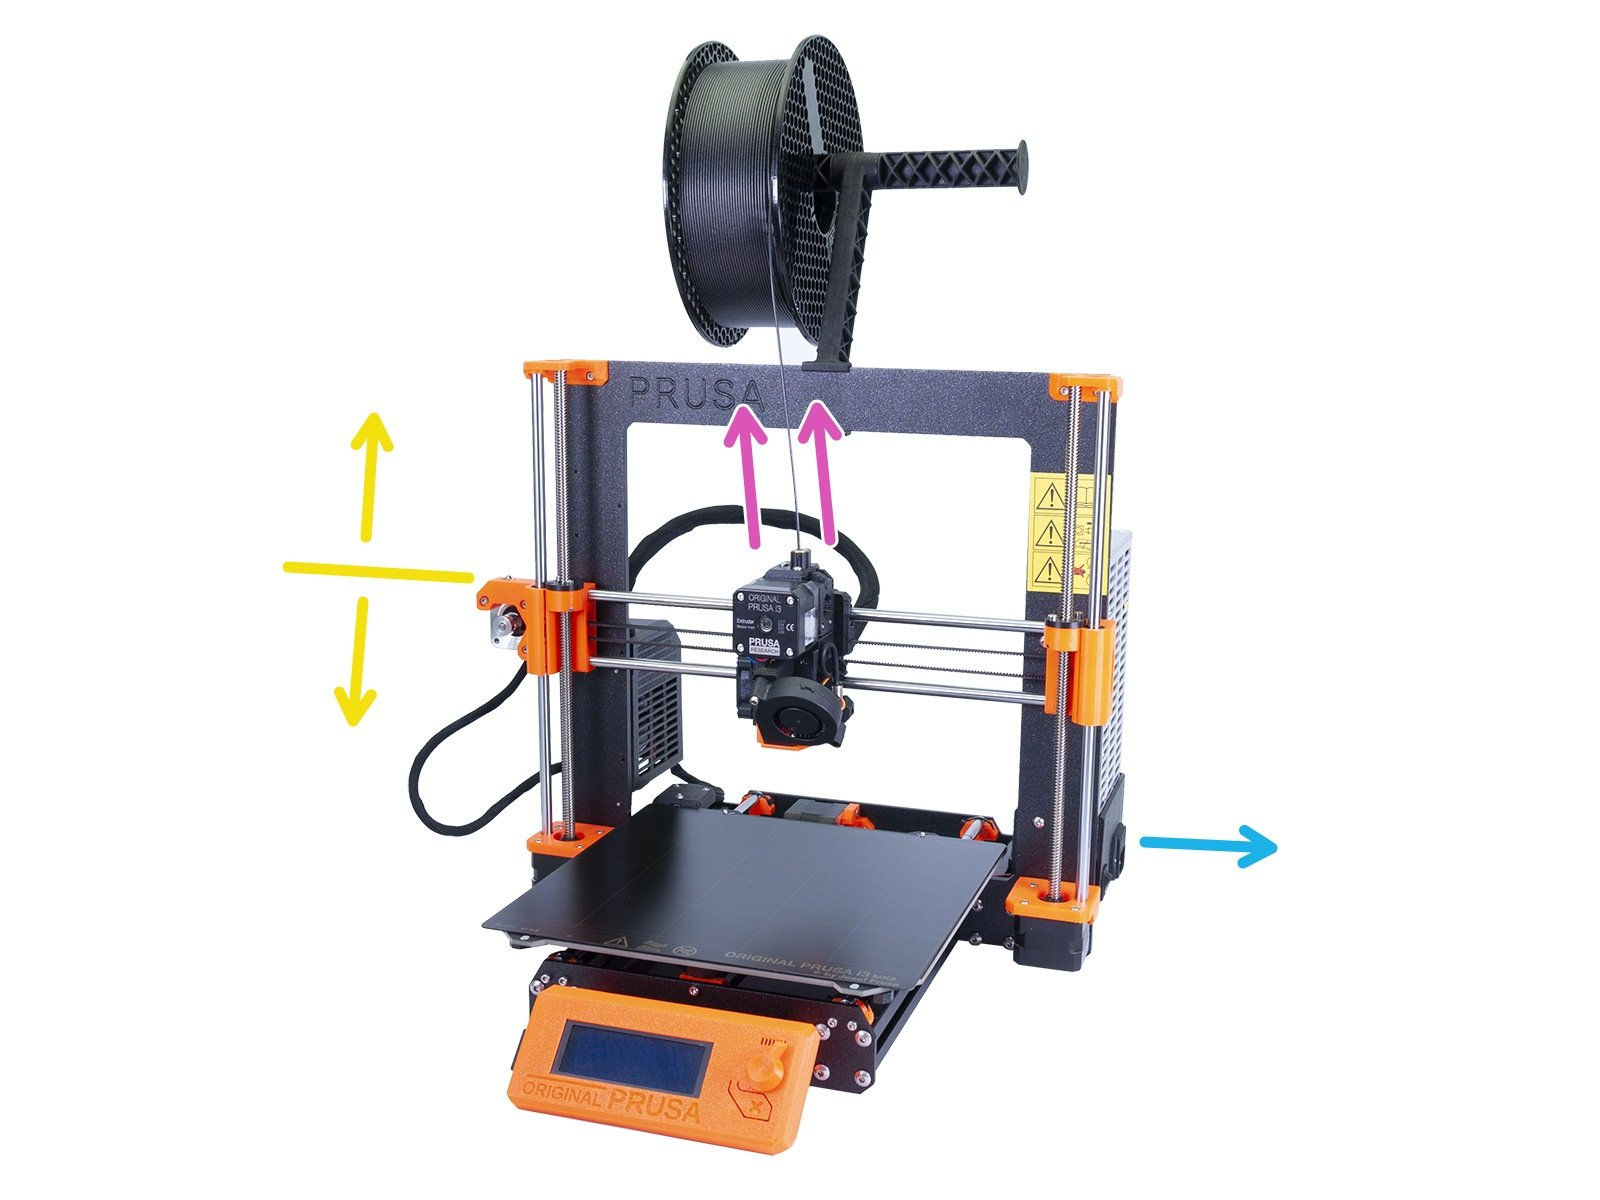
\includegraphics[width=0.5\linewidth]{bilder/Anleitung - X-Achse hoch.jpg}
              \caption[Anleitung: X-Achse auf die Hälfte der Gesamthöhe fahren] { X-Achse auf die Hälfte der Gesamthöhe fahren (Quelle: \autocite{Prusa})}
        \label{X-Achse hoch}
      \end{figure}
      \FloatBarrier
    \item Nun folgt das entfernen der Schrauben. Zunächst werden die in \autoref{Schraubi1} dargestellten Schrauben gelöst und entfernt. Im Anschluss werden die grün markierten Schrauben aus \autoref{Schraubi2} entfernt. Abschließend gilt es die orange markierten Schrauben, die den Extruder halten, aus \autoref{Schraubi3} zu entfernen.
      \begin{figure}[h] 
        \centering
        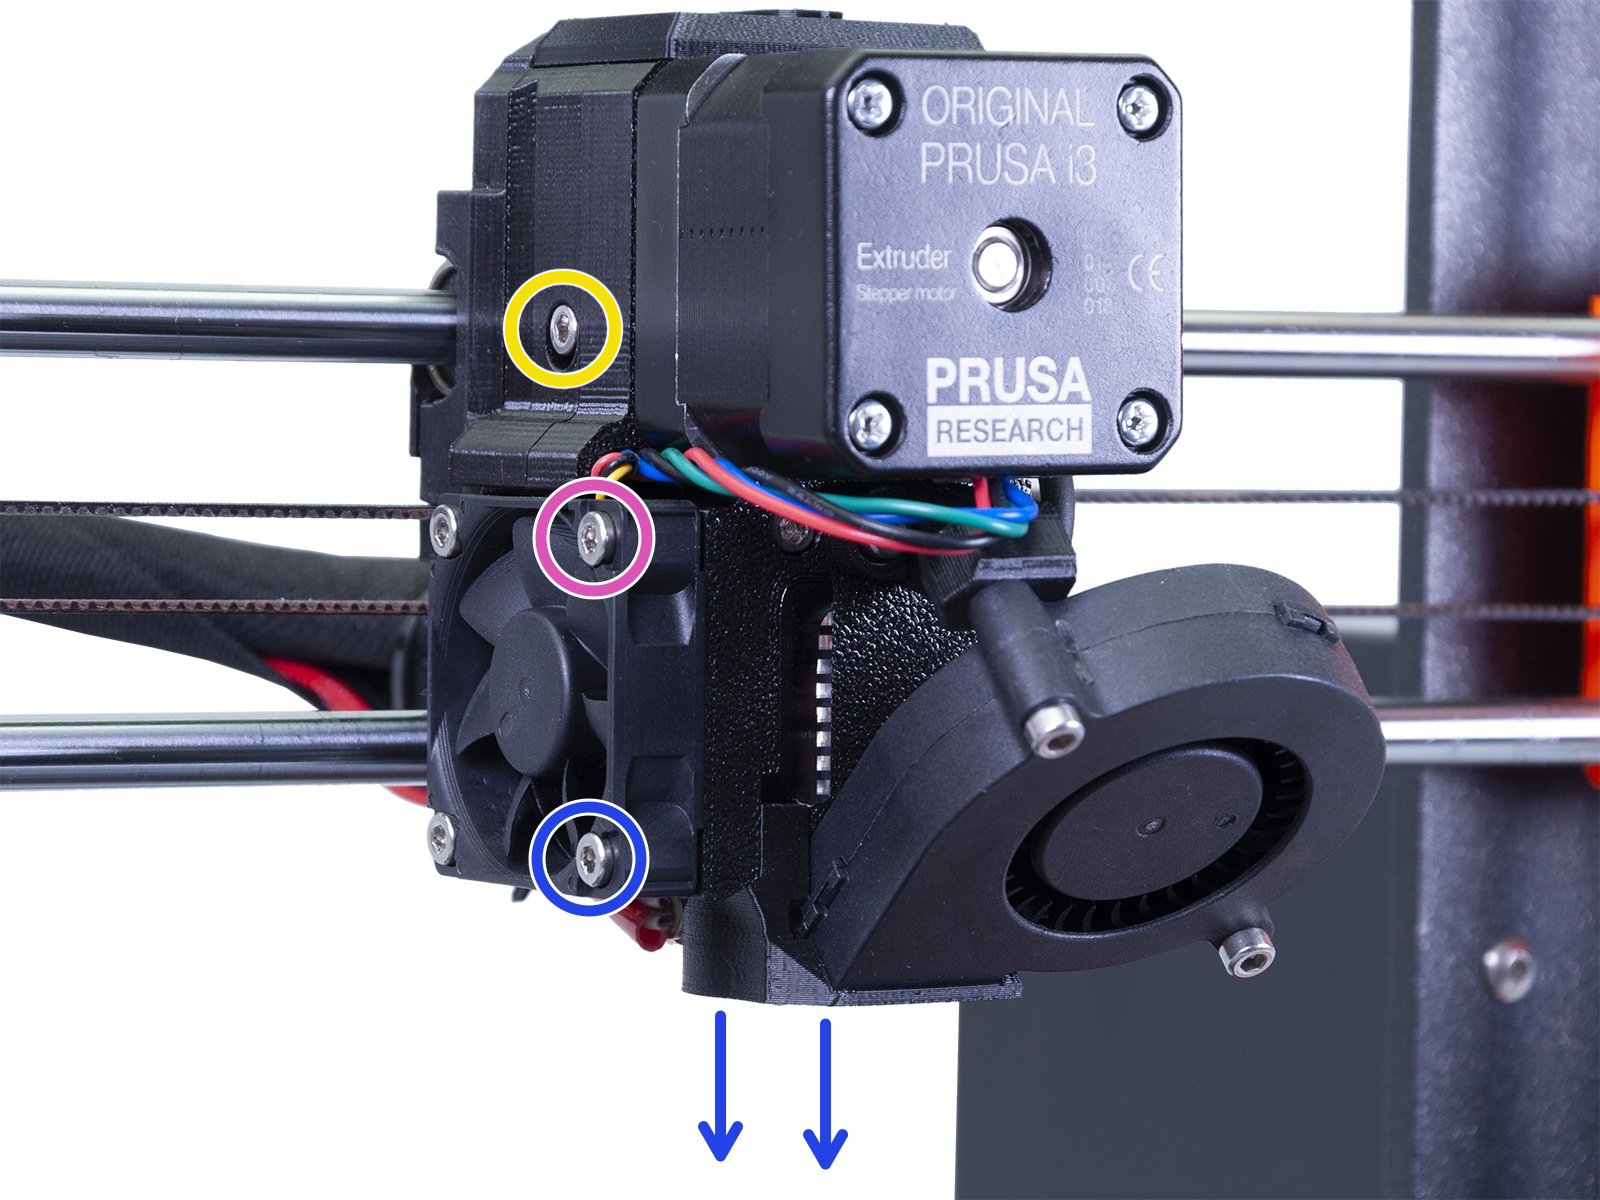
\includegraphics[width=0.5\linewidth]{bilder/Anleitung - Schraubi1.jpg}
              \caption[Anleitung: Gelb, lila und blau markierten Schrauben entfernen] {Gelb, lila und blau markierten Schrauben entfernen (Quelle: \autocite{Prusa})}
        \label{Schraubi1}
      \end{figure}
      \FloatBarrier
      \begin{figure}[h]
        \centering
        \begin{subfigure}[b]{0.45\textwidth}
          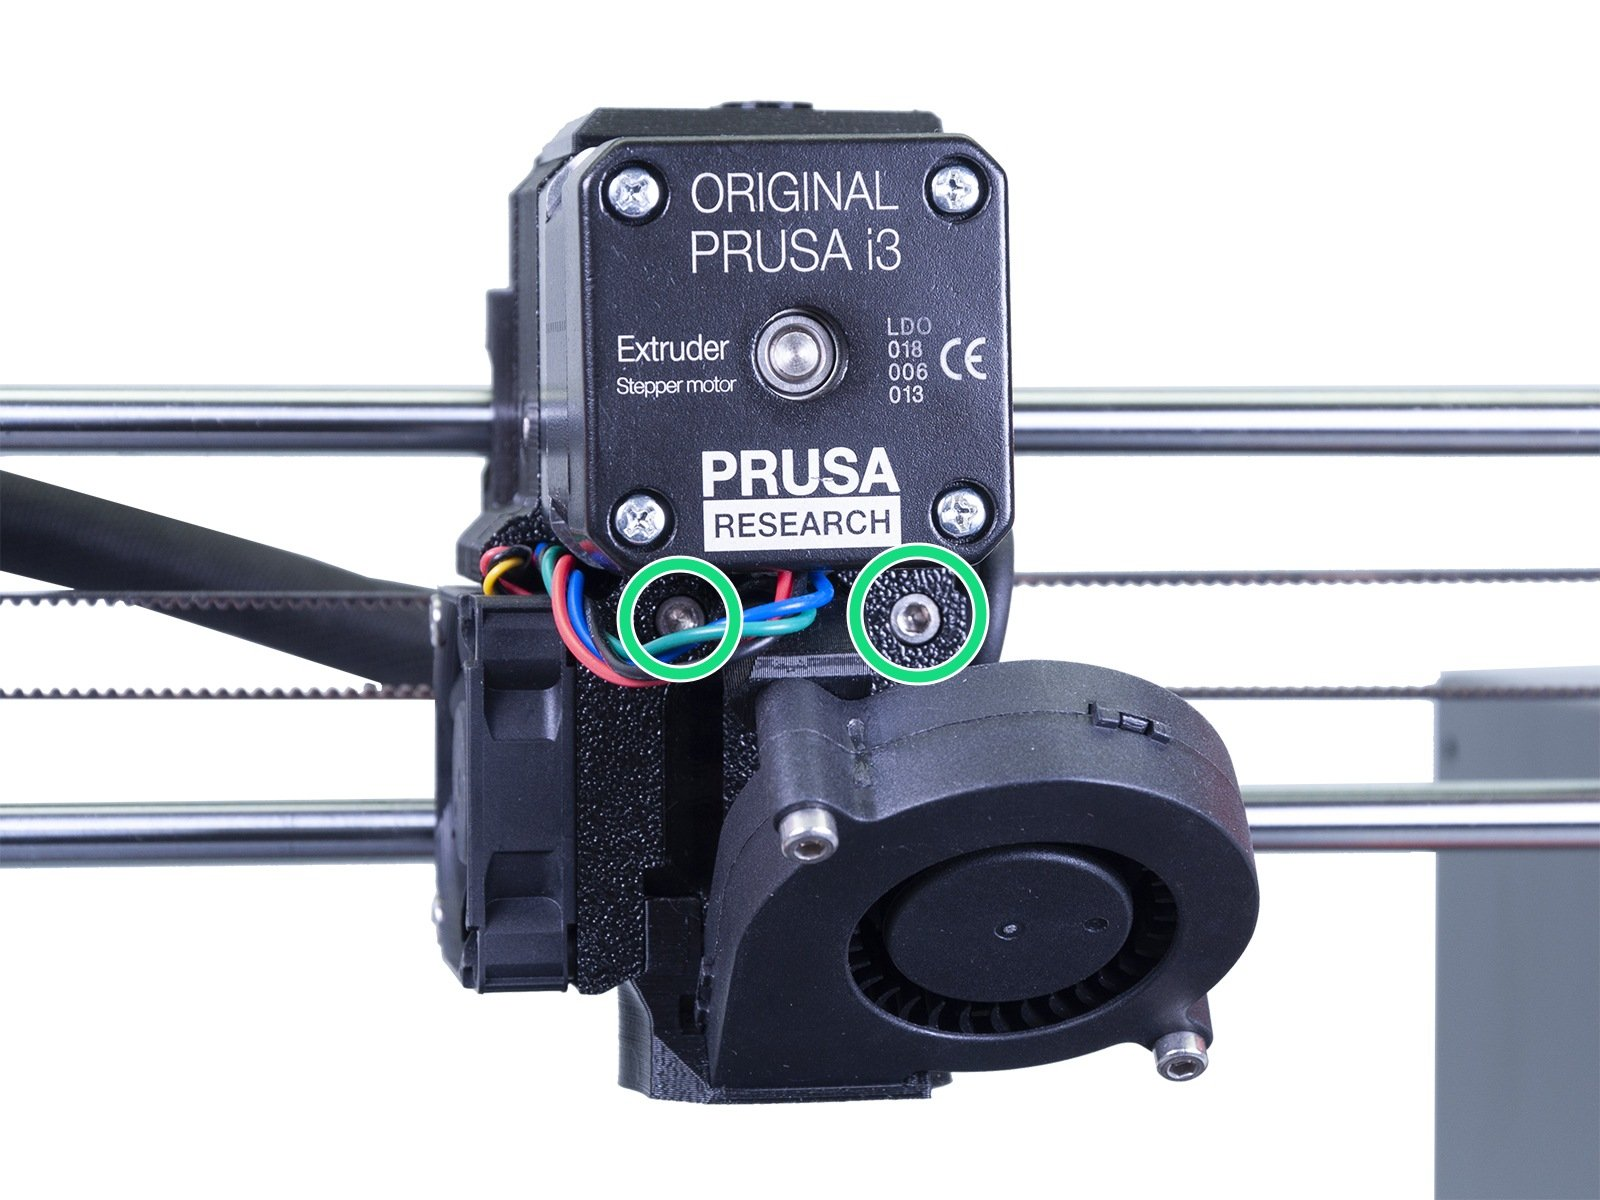
\includegraphics[width=\textwidth]{bilder/Anleitung - Schraubi2.jpg}
          \caption[Anleitung: Grün markierte Schrauben entfernen] {Grün markierte Schrauben entfernen (Quelle: \autocite{Prusa})}
          \label{Schraubi2}
        \end{subfigure}
        \hfill
        \begin{subfigure}[b]{0.45\textwidth}
          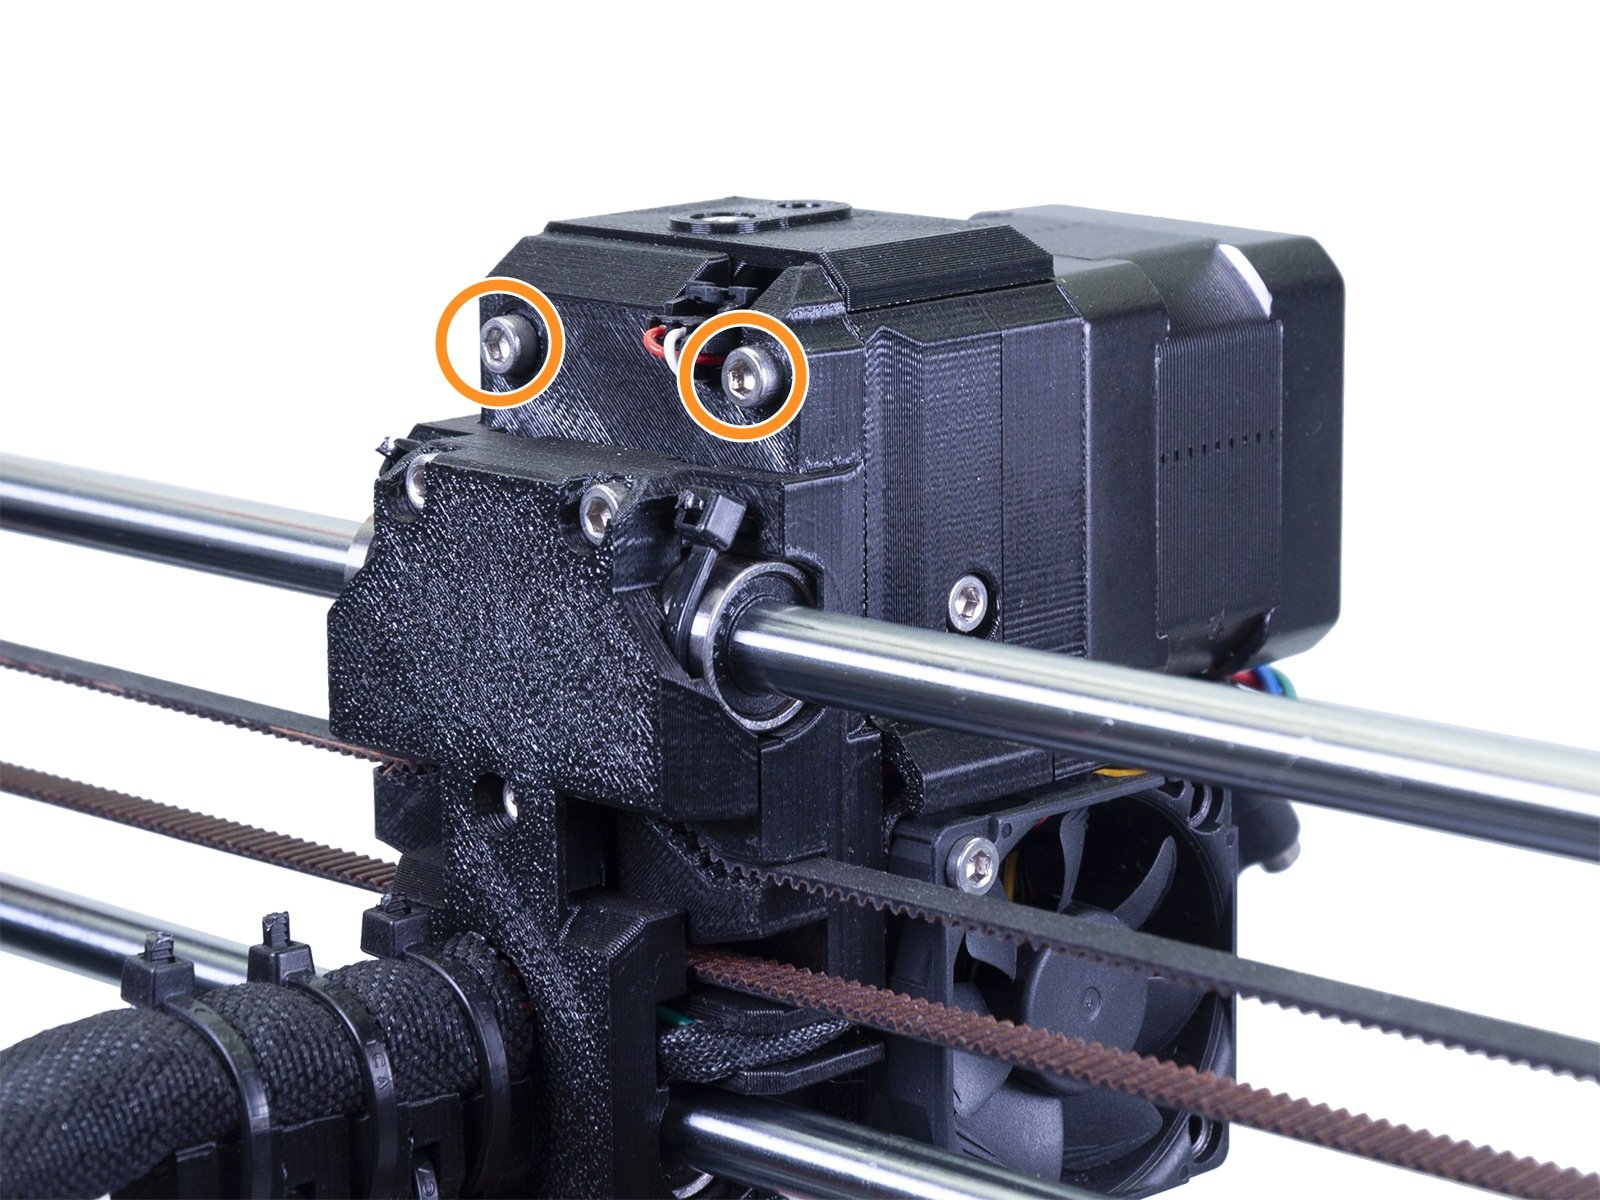
\includegraphics[width=\textwidth]{bilder/Anleitung - Schraubi3.jpg}
          \caption[Anleitung: Orange markierte Schrauben entfernen] {Orange markierte Schrauben entfernen (Quelle: \autocite{Prusa})}
          \label{Schraubi3}
        \end{subfigure}
      \end{figure}
      \FloatBarrier

    \item In diesem Schritt wird der Extruder teildemontiert. Dazu Wird vorsichtig der Extrudermotor in Pfeilrichtung (siehe \autoref{Zerlegen1}) gezogen. Sobald dieser lose ist, wird der untere Teil mit herausgezogen. Es muss eine Lücke, wie in \autoref{Zerlegen1} in gelb dargestellt, zu sehen sein.\\
          Nun kann das Hotend vorsichtig von unten entnommen werden (siehe \autoref{Zerlegen2}). Dabei auf die Kabel des Hotends achten, sie dürfen nicht beschädigt werden.
      \begin{figure}[h] 
        \centering
        
      \end{figure}
      \begin{figure}[h]
        \centering
        \begin{subfigure}[b]{0.45\textwidth}
          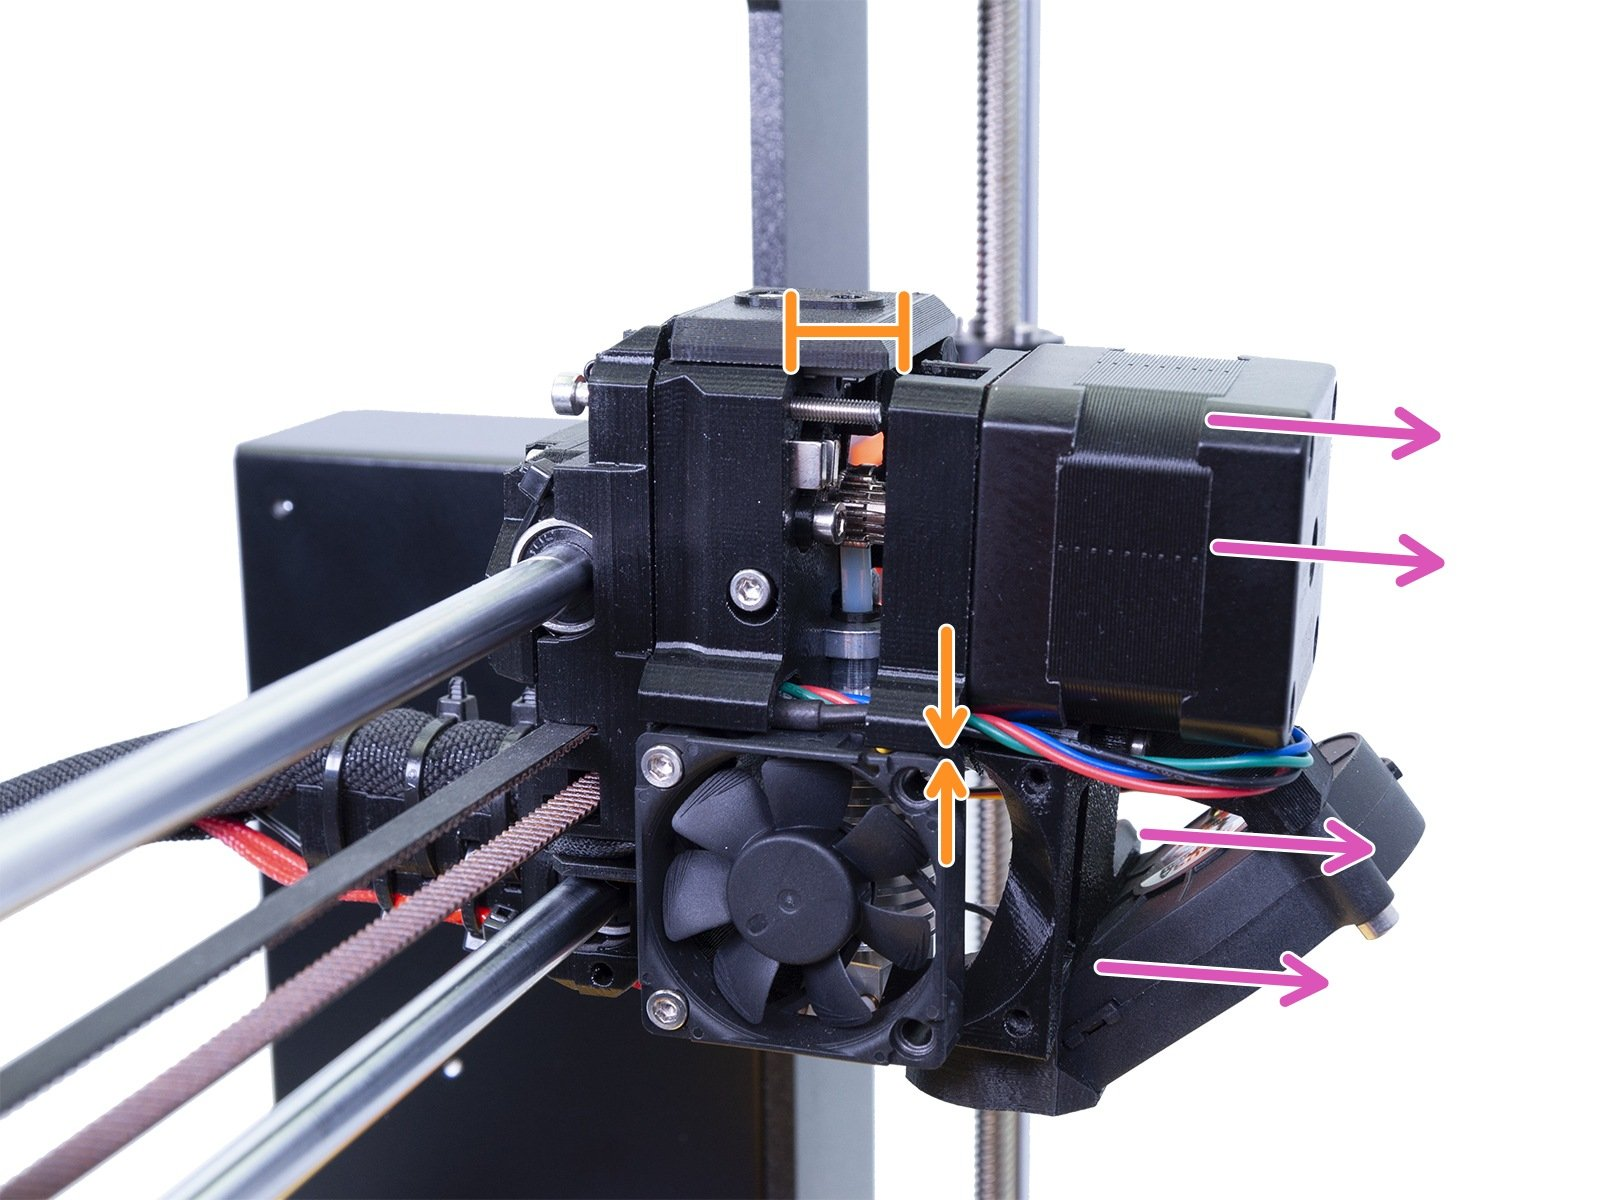
\includegraphics[width=0.5\linewidth]{bilder/Anleitung - Zerlegen1.jpg}
          \caption[Anleitung: Zerlegung des Extruders] {Zerlegung des Extruders (Quelle: \autocite{Prusa})}
        \label{Zerlegen1}
        \end{subfigure}
        \hfill
        \begin{subfigure}[b]{0.45\textwidth}
          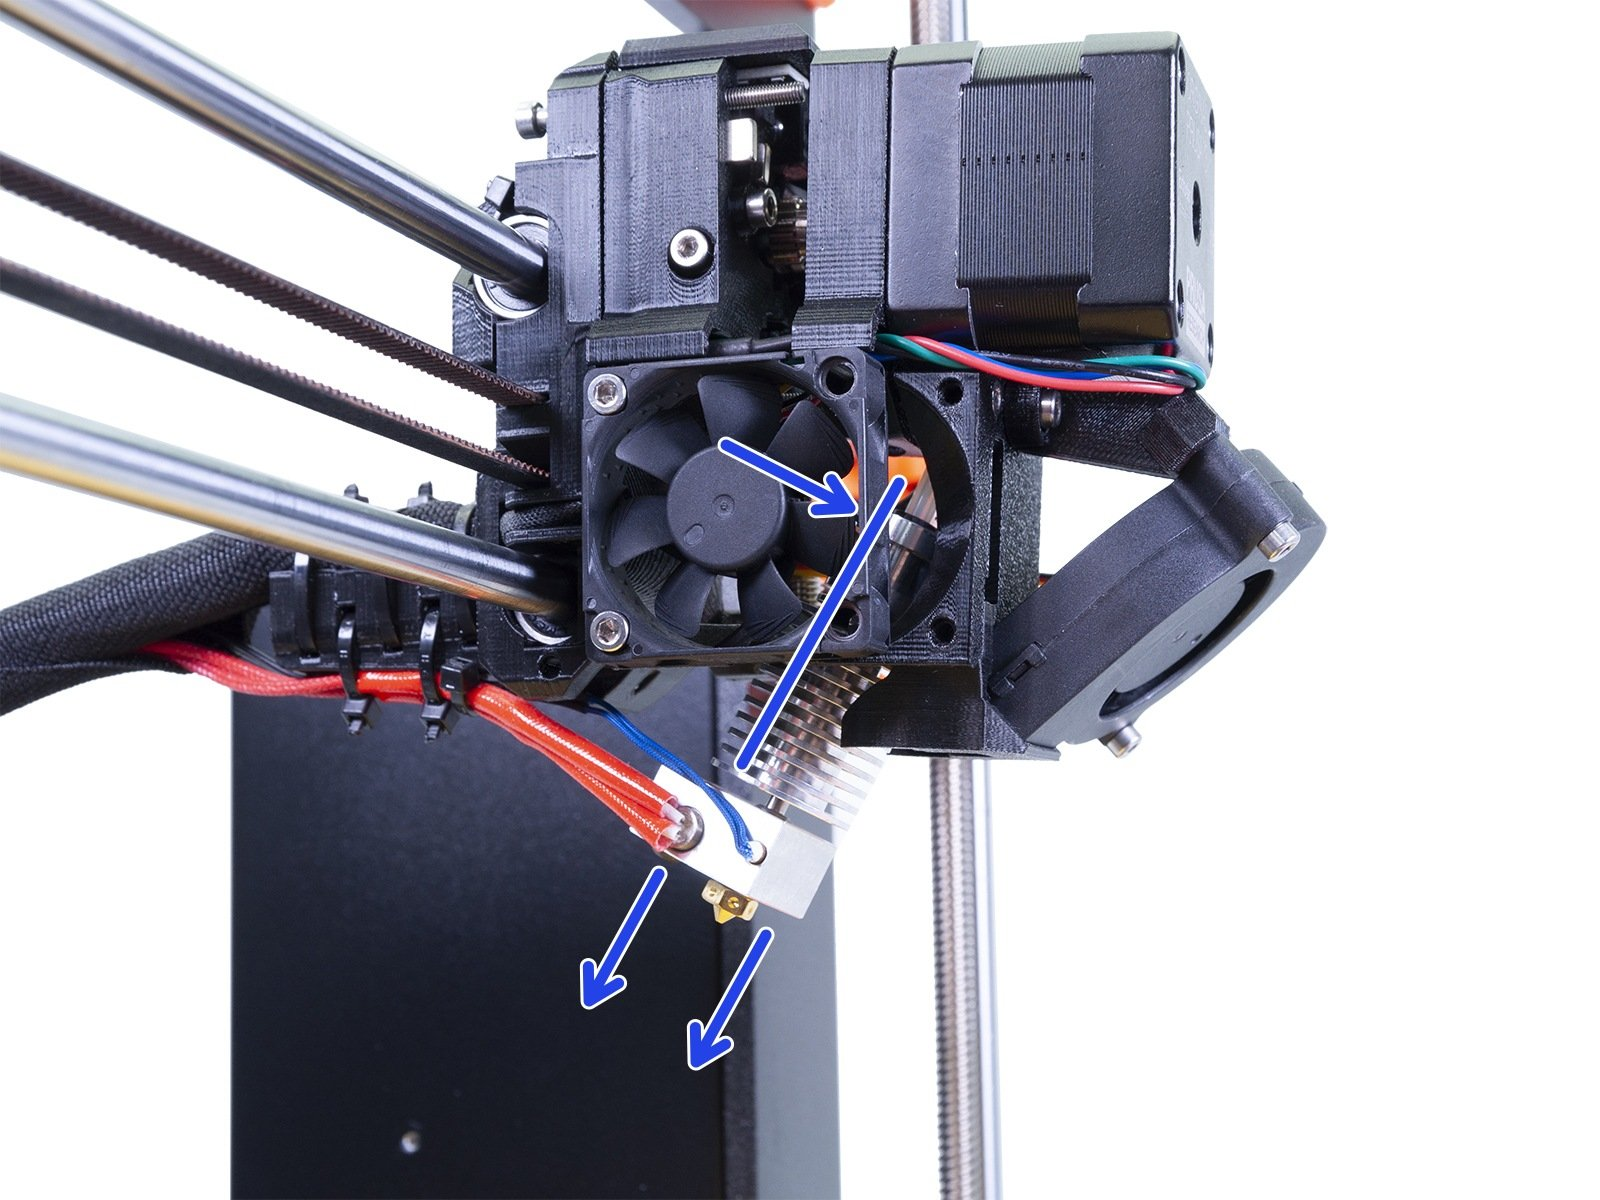
\includegraphics[width=\textwidth]{bilder/Anleitung - Zerlegen2.jpg}
          \caption[Anleitung: Vorsichtige Entnahme des Hotends] {Vorsichtige Entnahme des Hotends (Quelle: \autocite{Prusa})}
          \label{Zerlegen2}
        \end{subfigure}
      \end{figure}
      \FloatBarrier

    \item Jetzt kann das PTFE-Schlauchstück mithilfe der entfernt werden. Dazu mit den Fingern den, in \autoref{PTFEEE} mit blauem Pfeil markierten, Ring herunterdrücken und den Schlauch mit der beiliegenden Zange herausziehen. Nun kann die Verstopfung in diesem Schlauchstück mit einem langen, dünnen Hilfsmittel (z.B. einem Imbussschlüssel) entfernt werden.
      \begin{figure}[h] 
        \centering
        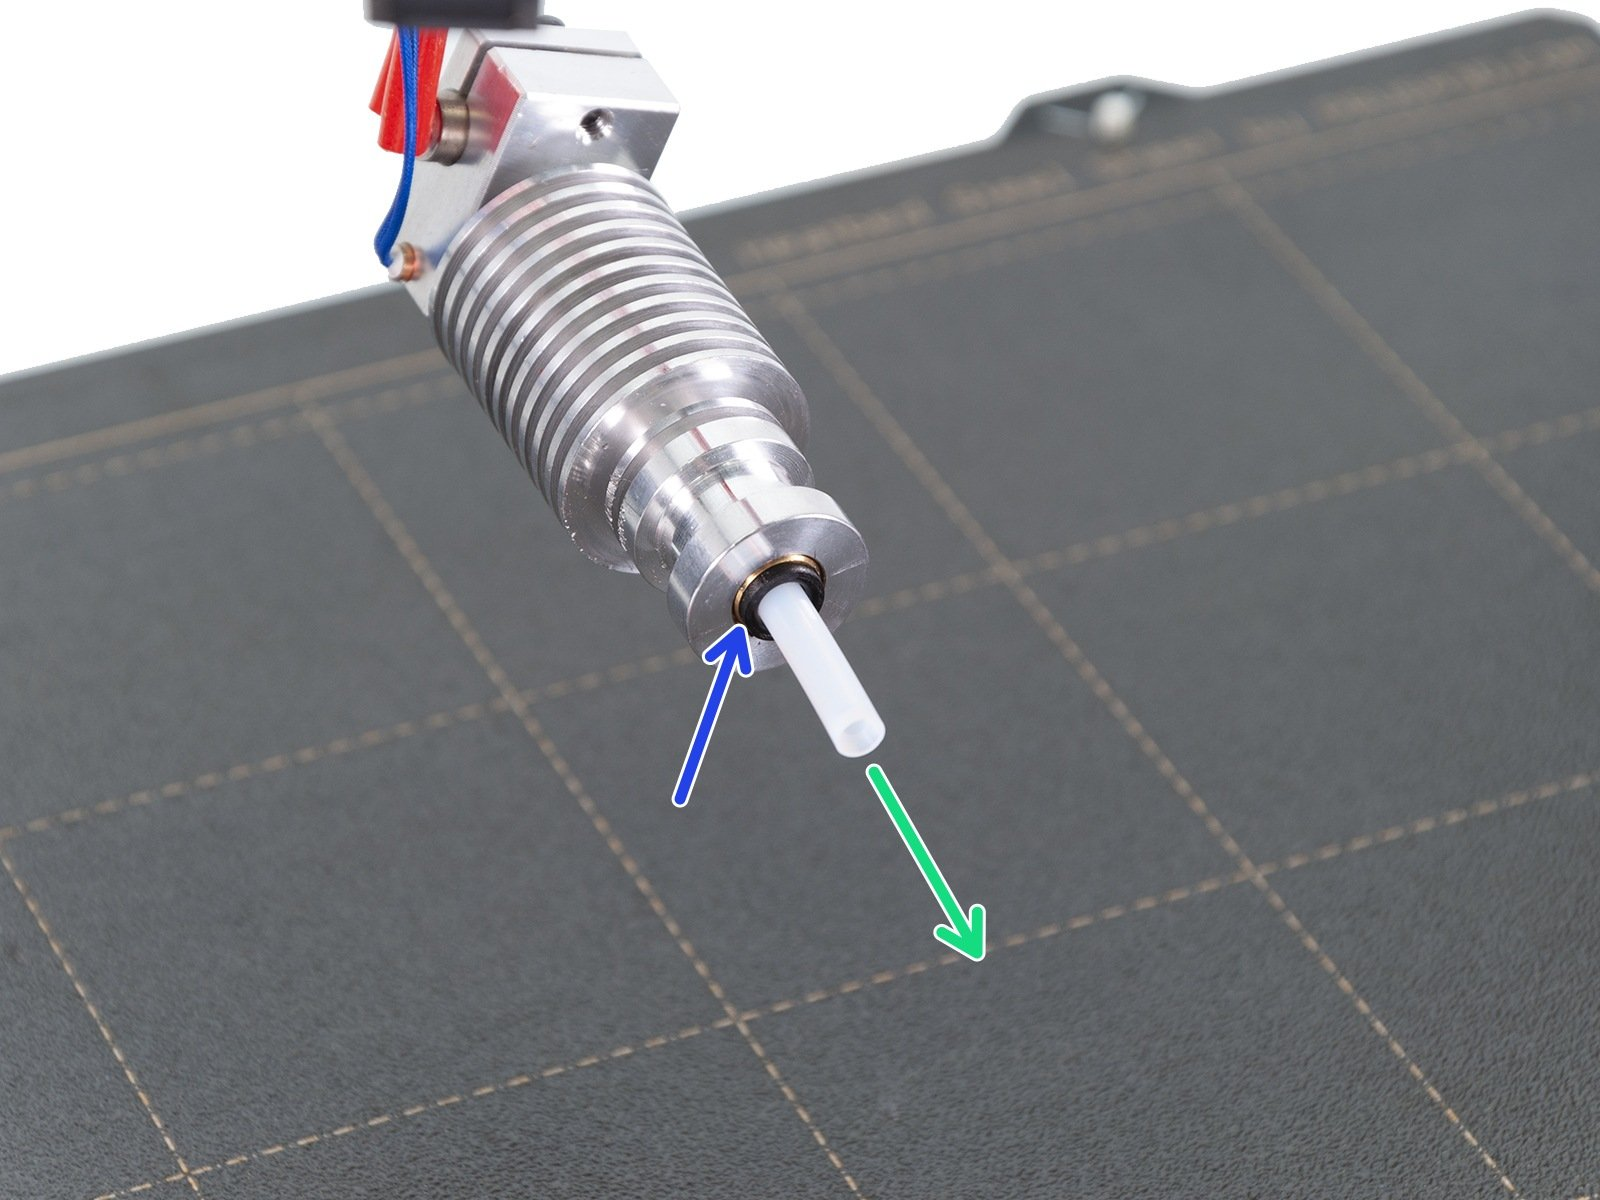
\includegraphics[width=0.5\linewidth]{bilder/Anleitung - Entfernen des PTFE-Schlauchs.jpg}
              \caption[Anleitung: Entfernen des PTFE-Schlauchstücks] {Entfernen des PTFE-Schlauchstücks (Quelle: \autocite{Prusa})}
        \label{PTFEEE}
      \end{figure}
      \FloatBarrier

    \item Der Zusammenbau geschieht in umgekehrter Reihenfolge. Wichtig ist, dass der PTFE-Schlauch mit dem angespitztem Ende wieder in den Extruder hineingeführt wird.
    \item Die in gelb dargestellte Schra
    \item Wenn alle Teile wieder zusammengebaut und die Schrauben wieder festgezogen sind, kann die Düse auf 180°C aufgeheizt werden. Sobald die Temperatur erreicht ist, wird das Ende der Filamentrolle schräg mit der Zange abgeschnitten. Um das  
\end{itemize}